% \documentclass{article}
\documentclass[12pt]{article}

% Language setting
% Replace `english' with e.g. `spanish' to change the document language
\usepackage[english]{babel}

% Set page size and margins
% Replace `letterpaper' with `a4paper' for UK/EU standard size
\usepackage[a4paper,top=2cm,bottom=2cm,left=2cm,right=2cm,marginparwidth=1.75cm]{geometry}
\usepackage{fontspec}
% 设置整个文档的主字体
\setmainfont{Times New Roman}
\linespread{1.0}




\RequirePackage{multirow}  % 列合并需要的宏包
\RequirePackage{array}	   % 对齐相关的宏包
\RequirePackage{booktabs}  % 三线表宏包
\RequirePackage{tabularx}  % 自动平均分配列宽的宏包
\RequirePackage{longtable} % 跨页表格需要的宏包
\RequirePackage{tabu}      % 大表格需要的宏包
\RequirePackage{threeparttable} % 三段式表格,主要用于表格内引用
\usepackage{graphicx}  % To allow using '\resizebox'
\usepackage{makecell}  % To allow multi-line cells and vertical centering
\usepackage{subcaption}
\usepackage{caption}
\usepackage{xcolor}

% Useful packages
\usepackage{pgf-pie}
\usepackage{geometry}
\usepackage{amsmath}
\usepackage{graphicx}
\usepackage[colorlinks=true, linkcolor=blue,backref=true]{hyperref}
\usepackage[hyperref=true,backref=true,style=apa, backend=biber,isbn=true]{biblatex}
\addbibresource{refinfo.bib}
\usepackage{pgfplots}
\pgfplotsset{compat=1.18}

\usepackage{array}
\usepackage{geometry}
\usepackage{longtable}
\usepackage{lscape}
% 新定义的列类型
\newcolumntype{L}[1]{>{\raggedright\arraybackslash}m{#1}} % 左对齐
\newcolumntype{C}[1]{>{\centering\arraybackslash}m{#1}}   % 居中对齐
\newcolumntype{R}[1]{>{\raggedleft\arraybackslash}m{#1}}  % 右对齐

\newcolumntype{P}[1]{>{\centering\arraybackslash}p{#1}}

\newcommand{\keywords}[1]{
    \vspace{1em} % 给关键字和摘要之间一些距离
    \noindent\textbf{Keywords:} {\fontsize{10pt}{12pt}\selectfont #1}
}



% for the f**king color
\usepackage{xcolor}
\newif\ifColorOn
\ColorOntrue
\ifColorOn
    % COLORFUL !!! WTF
    \definecolor{color-fxz}{HTML}{512DA8} % purple
    \definecolor{color-dbh}{HTML}{455A64} % grey
    \definecolor{color-zym}{HTML}{3F51B5} % indigo
    \definecolor{color-xdz}{HTML}{5D4037} % brown

\else
    % all black
    \definecolor{color-fxz}{rgb}{0, 0, 0}
    \definecolor{color-dbh}{rgb}{0, 0, 0}
    \definecolor{color-xdz}{rgb}{0, 0, 0}
    \definecolor{color-zym}{rgb}{0, 0, 0}
\fi

\title{\textbf{Utilizing Generative AI for Personalized Learning in Computer Science Education}}
\author{Baihan Deng, Daozheng Xue, Xiaoze Fan, Yumin Zhuang\footnote{Task assignment\\
\textcolor{color-dbh}{Baihan Deng: introduction \& conclusion  \textbf{grey}}
\\ 
\textcolor{color-xdz}{Daozheng Xue: discussion \textbf{brown}} \\ 
\textcolor{color-fxz}{Xiaoze Fan: abstract \& methodology \& technology support \textbf{purple}} \\
\textcolor{color-zym}{Yumin Zhuang: results \& questionnaire \& technology support \textbf{indigo}}\\
Some of the work is done by generative AI tools, including some sentences but mainly tedious technical work such as data analyzer programming and latex code generation for tikz figures.
}}

\begin{document}
\maketitle

\color{color-fxz}
\begin{abstract}
Generative Artificial Intelligence (GenAI) systems have experienced rapid growth in recent years, significantly impacting the educational field by offering capabilities such as paper writing, code generation, and concept explanation. Computer science (CS) students are at the forefront of adopting and benefiting from AI technologies, so it is crucial to understand how GenAI can specifically support CS education. This study explores the role of GenAI in assisting the personalized learning of CS students. By surveying 101 CS students from Shanghai Jiao Tong University (SJTU), we investigated their knowledge, usage, trust, and perceptions of AI tools in coding and learning tasks. Our results revealed diverse usage patterns and varying levels of trust in GenAI among students. Based on these findings, we discussed strategies to guide CS students to effectively utilize AI for personalized learning, considering their unique characteristics and needs. Overall, this research contributes to understanding CS students' perspectives on GenAI and offers recommendations for its effective integration into their personalized learning journeys.
\end{abstract}
\color{black}
\keywords{Education, Generative AI, Computer Science}

\newpage
\tableofcontents
\label{toc_contenttable}
\newpage

\color{color-dbh}
\section{INTRODUCTION}
\paragraph{}
Considering GenAI's huge effect in the future, it is very important to discuss how AI can help students appropriately, and those CS students who have been helped by GenAI can take part in GenAI's development in return, so it is also an interesting topic. In previous research, we find that some studies focus on the practicality of AI-assisted programming and examine professional programmers' perspectives on it, like ``A Large-Scale Survey on the Usability of AI Programming Assistants: Successes and Challenges."(\cite{liang-2023-LargeScaleSurveyUsability}) and ``Expectation vs. Experience: Evaluating the Usability of Code Generation Tools Powered by Large Language Models"(\cite{vaithilingam-2022-ExpectationVsExperience}).

\paragraph{}
Some studies focus on the general impact of generative AI on education, like ``Students' use of large language models in engineering education: A case study on technology acceptance, perceptions, efficacy, and detection chances"(\cite{bernabei-2023-StudentsUseLarge}) and ``With Great Power Comes Great Responsibility!': Student and Instructor Perspectives on the influence of LLMs on Undergraduate Engineering Education"(\cite{joshi-2023-GreatPowerComes}).

\paragraph{}
Others pay attention to exploring AI-assisted computer education(``Beyond Traditional Teaching: Large Language Models as Simulated Teaching Assistants in Computer Science"(\cite{liu-2024-TraditionalTeachingLarge})), exploring the possibility of AI teaching assistants from an educator's perspective(``Bob or Bot: Exploring ChatGPT's Answers to University Computer Science Assessment"(\cite{richards-2024-BobBotExploring}) and ``ChatGPT in the Classroom: An Analysis of Its Strengths and Weaknesses for Solving Undergraduate Computer Science Questions"(\cite{joshi-2024-ChatGPTClassroomAnalysis})) or testing AI in answering CS-related questions, investigating the extent of students' trust in AI(``Trust in Generative AI among Students: An exploratory study"(\cite{amoozadeh-2024-TrustGenerativeAI})).

\paragraph{}
In summary, the previous studies pay much attention to GenAI's effect on education generally, however, we find few studies take research on CS students specifically—hard-to-begin major students. As a group whose major is related to AI, it is hard to say whether these students' trust level in GenAI is the same as other students'. Also, considering different learning content, it remains unknown whether the general study method(with GenAI) suits the CS student. So in this article, we'll discuss how students and instructors trust GenAI and how to guide CS students to use GenAI to assist their personalized learning, in the hope of giving CS students some advice through our study.

\color{black}

\color{color-fxz}
\section{METHODOLOGY}
\paragraph{}
The methodology for this study is designed to evaluate the impact of generative AI (GenAI) tools on personalized learning within computer science (CS) education. To ensure a comprehensive understanding, the data collection and analysis approach integrates both quantitative and qualitative methods.

\subsection{Survey Design}
\paragraph{}
A structured questionnaire was developed to gather detailed insights from computer science students regarding their use and perceptions of generative AI tools. The questionnaire includes both closed and open-ended questions, addressing various aspects of GenAI usage in CS educational settings.

\paragraph{}
The survey questionnaire is divided into five parts:
\begin{enumerate}
    \item \textbf{Understanding and Usage} This section includes questions about participants' understanding of GenAI and the frequency of its use in their learning. These questions categorize participants into users and non-users of GenAI.
    \item \textbf{Application and Acceptance} This section explores how participants use GenAI, including the specific aspects of their studies where they employ generative AI, their level of acceptance towards AI-assisted learning, and whether AI has enhanced their efficiency.
    \item \textbf{Trust} This section assesses the participants' trust in GenAI, using three targeted questions to address various levels of trust.
    \item \textbf{Concerns} This section addresses participants' concerns about GenAI, such as data privacy, security issues, and potential negative impacts on skill development.
    \item \textbf{Additional Opinions} This final part includes an open-ended question for participants to share any additional opinions on the use of GenAI in CS learning.
\end{enumerate}

\paragraph{}
By structuring the survey in this manner, we aim to acquire a comprehensive understanding of participants' opinions on using GenAI in CS learning. Most of the questions are multiple-choice, with four options provided for frequency or degree measurements. For questions regarding reasons and aspects, multiple choices are available, along with an ``Other" option for additional inputs. This design facilitates quantitative analysis of the responses.

\subsection{Data Collection}

\paragraph{}
To gather comprehensive data for this study, we created a detailed electronic questionnaire and distributed it on the ShuiYuan forums of Shanghai Jiao Tong University (SJTU). To incentivize participation and obtain a higher response rate, we offered a small monetary reward to each participant. This approach was aimed at ensuring sufficient engagement and a broad representation of computer science students at various levels of study.

\color{black}

\color{color-zym}
\section{RESULTS}
\paragraph{}
During our study, we used the Wen Juan Xing platform to distribute the questionnaire. After about 3 days, we received 101 valid responses from CS students in different provinces ranging from freshmen to graduates. The table \ref{table:response_distribution} lists the Distribution of Survey Responses by Academic Level.

\begin{table}[ht]
\centering
\captionsetup{labelfont={bf},textfont={bf}}
\caption{\label{table:response_distribution}\textbf{Distribution of Survey Responses by Academic Level}}
\begin{tabular}{>{\raggedright}p{4cm}rr}
\toprule
Student levels & Subtotal & Proportion \\
\midrule
Freshman & 51 & 50.50\% \\
Sophomore & 18 & 17.82\% \\
Junior & 11 & 10.89\% \\
Senior & 5 & 4.95\% \\
Graduate & 16 & 15.84\% \\
\midrule
Total Valid Responses & \textbf{101} & \\
\bottomrule
\end{tabular}
\end{table}

\subsection{Students' Knowledge About AI}
\paragraph{}
As for their knowledge about generative AI tools such as ChatGPT, 42.57\% of respondents reported having a general understanding, while 47.52\% reported being familiar with these tools (Figure \ref{fig:understanding}). Only 9.9\% said they were not familiar with generative AI. This result suggests that the majority of computer science students surveyed have a basic understanding of generative AI technologies, which may contribute to their willingness to adopt these tools in their learning process.
\begin{figure}[h!]
    \centering
    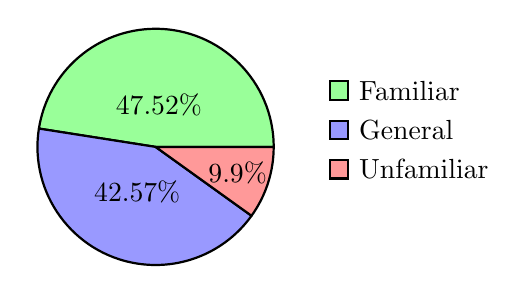
\begin{tikzpicture}
        \pie[
            text=legend,
            radius=1.5,
            color={green!40, blue!40, red!40}
        ]{
            47.52/Familiar,
            42.57/General,
            9.9/Unfamiliar
        }
    \end{tikzpicture}
    \caption{Respondents' Level of Understanding of Generative AI}
    \label{fig:understanding}
\end{figure}
\subsection{Students' Usage of AI}
\paragraph{}
The majority of respondents (65.35\%) reported using generative AI frequently in their studies (Figure \ref{fig:usage_frequency}), while 23.76\% used it occasionally. Only 4.95\% reported never using generative AI. The main purposes for using these tools (Figure \ref{fig:usage_purposes}) included assisting with programming (68.75\%), writing papers (87.5\%), and solving learning problems (80.21\%). These results suggest that generative AI has become an integral part of many computer science students' learning strategies, with a wide range of applications in different aspects of their studies.
\begin{figure}[h!]
    \centering
    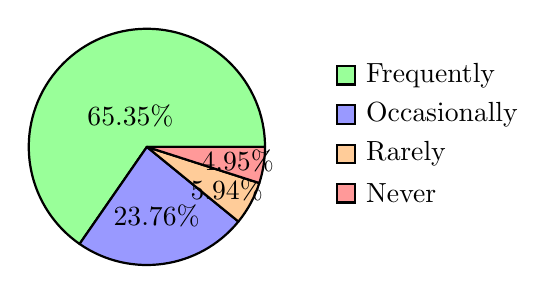
\begin{tikzpicture}
        \pie[
            text=legend,
            radius=1.5,
            color={green!40, blue!40, orange!40, red!40}
        ]{
            65.35/Frequently,
            23.76/Occasionally,
            5.94/Rarely,
            4.95/Never
        }
    \end{tikzpicture}
    \caption{Frequency of generative AI usage among respondents}
    \label{fig:usage_frequency}
\end{figure}

\begin{figure}
\centering
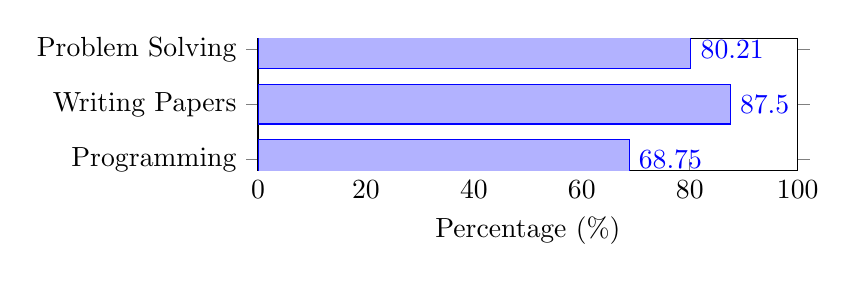
\begin{tikzpicture}
\begin{axis}[
    xbar,
    bar width=0.5cm,
    y=0.7cm,
    xmin=0,
    xmax=100,
    xlabel={Percentage (\%)},
    symbolic y coords={Programming, Writing Papers, Problem Solving},
    ytick=data,
    nodes near coords,
    nodes near coords align={horizontal},
    ]
\addplot coordinates {(68.75,Programming) (87.5,Writing Papers) (80.21,Problem Solving)};
\end{axis}
\end{tikzpicture}
\caption{Main purposes for using generative AI among respondents}
\label{fig:usage_purposes}
\end{figure}
\subsection{The Role AI Plays Among Students}
\paragraph{}
When asked about the helpfulness of generative AI in their learning, 45.54\% found it very helpful, and 37.62\% found it somewhat helpful. The main benefits reported (Figure \ref{fig:helpfulness_benefits}) were improved learning efficiency (82.18\%), expanded knowledge (49.5\%), enhanced programming skills (49.5\%), and others such as helping with creative inspiration (50.5\%) and providing learning resources (47.52\%). These results suggest that generative AI is playing a significant role in supporting and enhancing computer science students' learning experiences, with a majority of respondents recognizing its positive impact on various aspects of their academic development.
\begin{figure}
\centering
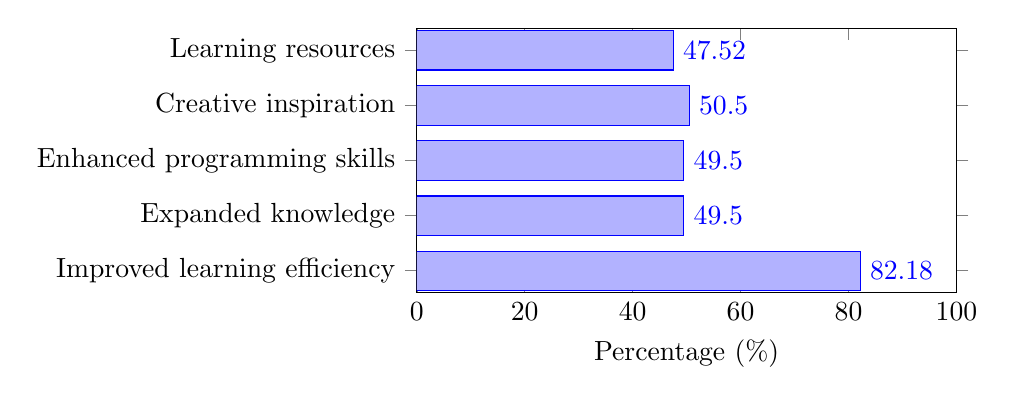
\begin{tikzpicture}
\begin{axis}[
    xbar,
    bar width=0.5cm,
    y=0.7cm,
    xmin=0,
    xmax=100,
    xlabel={Percentage (\%)},
    symbolic y coords={Improved learning efficiency, Expanded knowledge, Enhanced programming skills, Creative inspiration, Learning resources},
    ytick=data,
    nodes near coords,
    nodes near coords align={horizontal},
    ]
\addplot coordinates {(82.18,Improved learning efficiency) (49.5,Expanded knowledge) (49.5,Enhanced programming skills) (50.5,Creative inspiration) (47.52,Learning resources)};
\end{axis}
\end{tikzpicture}
\caption{Benefits of generative AI in computer science students' learning}
\label{fig:helpfulness_benefits}
\end{figure}
\subsubsection{Specific Performance of AI in Coding Tasks}
\paragraph{}
As for utilization of AI programming assistants like Copilot, 25.74\% of the respondents use AI frequently, while 26.73\% used them occasionally. This indicates that AI programming assistants are popular among computer science students and are perceived as useful tools for boosting coding productivity.

\paragraph{}
The following are the actual effects:
\begin{itemize}
    \item Regarding the impact of these tools on their programming efficiency, 30.19\% of the respondents thought AI contributed to a significant increase, and 45.28\% reported a moderate increase.
    \item Regarding the AI tools' correctness in coding tasks, 64.15\% of the respondents believed that AI helped them improve the correctness, while 26.42\% of the respondents experienced no noticeable impact.
    \item Regarding the influence on debugging efficiency, 43.56\% of the respondents believed that AI helped improve their debugging efficiency, while 48.51\% of the respondents experienced no noticeable impact.
\end{itemize}
\paragraph{}
These results suggest that AI programming assistants can enhance code quality and simplify the debugging process for a significant portion of students, although the extent of their impact may vary depending on subjective judgment and the specific tools used.

\subsection{Students’ Level of Trust in AI}
\subsubsection{The Scale of Their Trust}
\paragraph{}
Regarding the correctness of AI's explanations of concepts(Figure \ref{fig:ai_trust}), 57.42\% of respondents believed in AI's abilities (22.77\% strongly believed, 34.65\% believed), while 34.65\% were neutral. For AI's reasoning abilities, 49.5\% believed in AI (14.85\% strongly believed, 34.65\% believed), and 36.63\% were neutral. As for AI's creative abilities, 48.51\% believed in AI (13.86\% strongly believed, 34.65\% believed), while 35.64\% were neutral. The data suggests that the perception abilities of AI are widely acknowledged while the creative abilities are less trusted, which is consistent with our prediction.
\begin{figure}[h!]
    \centering
    \begin{subfigure}{0.32\textwidth}
        \centering
        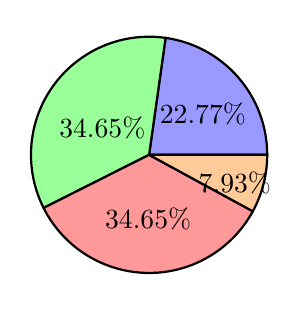
\begin{tikzpicture}
            \pie[
                text=inside,
                radius=1.5, % 半径为1.5厘米
                color={blue!40, green!40, red!40, orange!40}
            ]{
                22.77/,
                34.65/,
                34.65/,
                7.93/
            }
        \end{tikzpicture}
        \caption{Perception Abilities}
    \end{subfigure}
    \begin{subfigure}{0.32\textwidth}
        \centering
        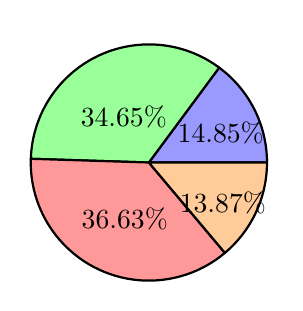
\begin{tikzpicture}
            \pie[
                text=inside,
                radius=1.5, % 半径为1.5厘米
                color={blue!40, green!40, red!40, orange!40}
            ]{
                14.85/,
                34.65/,
                36.63/,
                13.87/
            }
        \end{tikzpicture}
        \caption{Reasoning Abilities}
    \end{subfigure}
    \begin{subfigure}{0.32\textwidth}
        \centering
        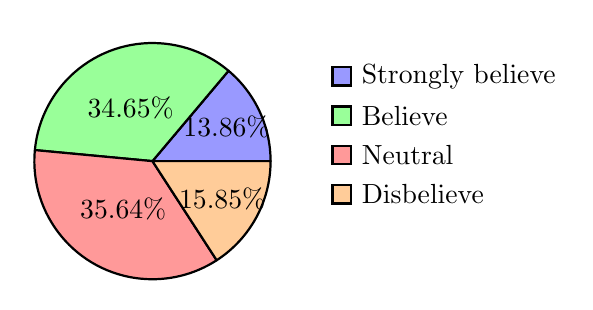
\begin{tikzpicture}
            \pie[
                text=legend,
                radius=1.5, % 半径为1.5厘米
                color={blue!40, green!40, red!40, orange!40}
            ]{
                13.86/Strongly believe,
                34.65/Believe,
                35.64/Neutral,
                15.85/Disbelieve
            }
        \end{tikzpicture}
        \caption{Creative Abilities}
    \end{subfigure}
    \caption{Respondents' Trust in Generative AI's Capabilities}
    \label{fig:ai_trust}
\end{figure}
\subsubsection{Why do They Hold That Belief}
\paragraph{}
A \textbf{qualitative} analysis of the data set suggests that students' level of trust in AI may have something to do with their knowledge about AI and the feedback from actual usage experiences. For example, students who know (and have access to) more advanced AI tools tend to rate higher trust levels. Also, students who enjoy huge benefits from AI tend to trust AI tools more as well.

\subsection{Quantitative Analysis of Relationship Between Effect and Trust}
\paragraph{}
In order to further talk about students' trust in AI, thus leading to how to utilize AI better, we need to investigate further into the relationship between effect and trust.
\paragraph{}
Take coding tasks for example, we can calculate the correlation coefficient matrix (Table \ref{table:correlation_matrix}). These results show that there is a positive correlation between AI's impact on code correctness and users' trust in the AI's ability to reason and create. In contrast, trust in conceptual explanations has almost no effect. This phenomenon suggests that students generally believe that the correctness of an AI's programming work has much to do with the AI's ability to reason and create. In other words, in order to improve students' trust in AI in the usage scenario of programming, we need to enhance AI's capability of reasoning and creating.

\begin{table}[h]
    \centering
    \renewcommand{\arraystretch}{2}
    \resizebox{\textwidth}{!}{
    \begin{tabular}{|c|c|c|c|c|}
        \hline
        \makecell{\\} & \makecell{perception abilities} & \makecell{reasoning abilities} & \makecell{creative abilities} & \makecell{code correctness} \\ \hline
        \makecell{perception abilities} & 1.000000   & 0.534916   & 0.317724   & 0.000587       \\ \hline
        \makecell{reasoning abilities} & 0.534916   & 1.000000   & 0.331429   & 0.341268       \\ \hline
        \makecell{creative abilities} & 0.317724   & 0.331429   & 1.000000   & 0.369839       \\ \hline
        \makecell{code correctness} & 0.000587 & 0.341268   & 0.369839   & 1.000000       \\ \hline
    \end{tabular}
    }
    \caption{Correlation coefficient between AI's influence on code correctness and trust in three levels of abilities}
    \label{table:correlation_matrix}
\end{table}

\subsection{Other Information}
\paragraph{}
Aside from the critical information mentioned above, we can retrieve other information from the questionnaire.
\paragraph{}
Regarding concerns about generative AI, 37.62\% of the respondents were worried about data privacy and security issues, while 52.48\% were not particularly concerned, and 9.9\% were not concerned at all. Judging from the results, we can say that while data privacy and security are important considerations for a significant portion of students, the majority do not view them as major barriers to using generative AI tools in their learning.

\paragraph{}
As for whether generative AI will negatively impact their skill development and employment prospects, 50.5\% of the respondents believed AI would not, while 12.87\% believed it would, and 36.63\% were not sure. The open-ended responses provided some insight into the reasons for these beliefs. Some students expressed concern that AI could replace certain job roles or lower the barrier to entry, leading to increased competition. Other respondents noted that AI could help automate low-level tasks, allowing students to focus on higher-level skills and adapt to the changing landscape of the computer science field.

\paragraph{}
These results provide a nuanced picture of computer science students' perceptions and experiences with generative AI in their learning. While the majority of respondents recognize the benefits and actively use these tools, there are still concerns and uncertainties that need to be addressed through further research, education, and guidance on the responsible and effective integration of AI in computer science education.



\color{black}

\color{color-xdz}
\section{DISCUSSION}
\subsection{How to Guide CS Students to Use AI to Assist Their Personalized Learning}
\subsubsection{The Feature of CS Students}

\paragraph{}
According to the general curriculum requirements of computer science, We focus our attention on the following aspects:
\paragraph{}
Need of knowledge from a wide range of fields. The knowledge of computer science is 
significantly different from other majors, Which is different from other traditional majors such as Physics and mathematics. In traditional majors, A comprehensive knowledge framework is usually constructed, and students start their learning by understanding the construction of this knowledge framework and gradually progress through it. But to a new CS student, the language is just like the basic rules, which cannot be Deductive reasoning by the existing knowledge. It is a system that is very rich and complex in content. And because of the dispersed characteristics of language, the importance of the search engine is vast. In that case, the effect of concise search is in need.
\paragraph{}
The practice of programming and debugging are the basic skills of CS students.
They all need students familiar with the programming language and the possible mistakes. But as the programming needs high accuracy, some mirror mistakes will cause a disaster. Maybe the mistake is obvious by the AI, but the students could not find it quickly. Then, The debug will cost a lot of meaningless time. Plus, repeated programming will also cost a lot of energy.
\subsection{The Recommendation of Learning with AI.}
\paragraph{}
According to our research, AI has already played an important role in the CS students’ study. A great part of students often use GenAI to assist with their studies (65.35 percent), and almost every student has the experience to use GenAI(95.15 percent). But when it comes to programming, the rate declines rapidly. Only 25.74 percent of students often use GenAI. The result reveals that AI has been widely used by CS students, but targeted applications of programming have not yet become widespread. So we will discuss some ways to use AI targeted for CS students.
\subsubsection{To Get Information More Efficiently and Targeted}
\paragraph{}
As we have discussed, The complex knowledge system is a feature of CS. While the traditional search engine is inefficient in front of the scattered knowledge, AI could efficiently retrieve and filter. In fact, Expanding one’s knowledge and providing learning resources is a common direction many students pursue when using AI (49.5 percent and 47.52 percent). Therefore, CS students should leverage AI’s concise search ability to find the most suitable learning materials and courses based on their individual needs and progress. AI recommendation can provide customized learning paths tailored to students’ learning history and interests.
\paragraph{}
Additionally, CS often needs creative solutions to a specific problem, which is the weakness of traditional search engines. Students can ask AI for some constructive suggestions, getting inspiration from the answers. Students can also ask AI about the motivations behind certain actions and
delve deeper into areas they do not understand, achieving in-depth and targeted learning.

\subsubsection{Programming Under the Assistance of AI May Be More Friendly to Beginners}
\paragraph{}
As programming and debugging are the most time-consuming parts of beginners' learning, They could apply AI to their daily work. According to our research, The majority of students agree that AI could enhance their programming and debug efficiency. It could be a powerful tool for beginners to finish their work. But to beginners, the most important thing is how to provide their skills. Enhancing the efficiency but not becoming an obstacle to them could be a future learning direction.

\color{black}

\color{color-dbh}
\section{CONCLUSION}
\paragraph{}
In conclusion, our study focuses on utilizing Generative AI for personalized learning in CS education, and through our study, we find out that it can benefit CS students a lot, as long as CS students correctly use it.
\paragraph{}
We found out that a large part of CS students know Generative AI and usually use it to help them complete tasks. While more than half of them believe in AI’s problem-solving ability, some of them do worry about data security.
\paragraph{}
% todo 给段首的几个结论找文献依据
Compared with all college students, CS students show higher usage frequency and trust levels about AI and lower worry levels about information leakage. This may be because their major is more relevant to this area. Through our study, we have further improved CS students’ views about Generative AI and relative things that haven’t been studied specifically.
\paragraph{}
What can not be ignored is that limited by limited time, allocation, and researchers, we only get about 100 answer sheets thus our discovery may have some degree of randomness. At the same time, we do not track students’ learning life so we do not get data about AI’s real influence on CS students in the long term.
\paragraph{}
However, our study does get data about CS students’ opinions on Generative AI. Based on the data we collect, we recommend that CS students should use Generative AI more targeted, and not worry about asking Generative AI to help you write, check, or explain your code. At the same time, we also hope that Generative AI can further strengthen the security of data.

\color{black}

\newpage
\appendix
% 调整表格间距
\setlength{\tabcolsep}{10pt} % 控制水平间距,值越大间距越大
\renewcommand{\arraystretch}{1.2} % 控制垂直间距,值越大间距越大
\section{DATA}
\footnotesize

The questionnaire: \textbf{Survey on the Opinions of Computer Science Students About Generative AI}

\begin{longtable}{L{.35\textwidth} L{.15\textwidth} L{.15\textwidth} L{.15\textwidth}}
    \hline
    \textbf{Questions} &\textbf{Options}  &  &  \\ \hline
    
    \textbf{1. What is your current academic year?} & Freshman & Sophomore & Junior \\
    & Senior & Graduate & \\ \hline
    
    \textbf{2. How well do you understand generative AI (e.g., ChatGPT, Claude, Gemini)?} & Familiar & General & Unfamiliar \\ \hline
    
    \textbf{3. Have you used generative AI tools during your studies?} & Frequently & Occasionally & Rarely \\
    & Never & & \\ \hline
    
    \textbf{4. What is your main purpose for using generative AI tools? (Select all that apply)} & Programming & Writing Papers & Solving Problems \\
    & Other & & \\ \hline
    
    \textbf{5. How helpful do you find generative AI for your studies?} & Very helpful & Helpful & Average \\
    & Not very helpful & Not helpful & \\ \hline
    
    \textbf{6. In what areas do you find generative AI most helpful in your studies? (Select all that apply)} & Improve Learning Efficiency & Enhance Programming Skills & Expand Knowledge \\
    & Aiding Creative Ideas & Providing Learning Resources & Other \\ \hline
    
    \textbf{7. Have you ever used AI programming assistance tools like Copilot when programming?} & Frequently & Occasionally & Never \\ \hline
    
    \textbf{8. Why haven't you used these tools?} & Haven't heard of them & I don't need them & Tried but couldn't access \\
    & Tried, but found them ineffective & & \\ \hline
    
    \textbf{9. How much do you think tools like Copilot improve your programming efficiency?} & Significantly & Moderately & Average \\
    & Negatively & & \\ \hline
    
    \textbf{10. How do you think tools like Copilot affect the correctness of your code?} & AI helps improve code correctness & No noticeable effect & Increases bugs \\ \hline
    
    \textbf{11. How do you think tools like Copilot affect your debugging efficiency?} & AI helps improve debugging efficiency & No noticeable effect & AI interferes with debugging \\ \hline
    
    \textbf{12. I trust the accuracy of AI's explanations of concepts (e.g., what is a pointer, what is a Turing machine)} & Strongly trust & Trust & Neutral \\
    & distrust & & \\ \hline
    
    \textbf{13. I trust AI's reasoning capabilities (e.g., which algorithm to use for solving a problem)} & Strongly trust & Trust & Neutral \\
    & distrust & & \\ \hline
    
    \textbf{14. I trust AI's creativity (e.g., writing a Turing machine simulator in C and running a+b on it)} & Strongly trust & Trust & Neutral \\
    & distrust & & \\ \hline
    
    \textbf{15. Do you think generative AI will negatively impact your skill development or job prospects?} & Yes & No & Uncertain \\ \hline
    
    \textbf{16. Why do you think it will have a negative impact?} & & & \\ \hline
    
    \textbf{17. Do you worry about data privacy and security issues when using generative AI tools?} & Worried & Somewhat worried & Not worried \\ \hline
    
    \textbf{18. Other thoughts:} &&& \\ \hline
\end{longtable}

The raw questionnaire and result can be found online at \\ \href{https://github.com/happyZYM/EnglishAcademicWriting-2024spring/raw/data/data.xlsx}{https://github.com/happyZYM/EnglishAcademicWriting-2024spring/raw/data/data.xlsx}.


\section{REFERENCES}
\nocite{*}
\printbibliography[heading=none]
\end{document}